\documentclass[11pt,letter]{article}
\usepackage[ a4paper,total={170mm,257mm},left=20mm,top=35mm]{geometry}
\usepackage{amsfonts}
\usepackage{amssymb}
\usepackage{amsthm}
\usepackage{amsmath}
\usepackage{newlfont}
\usepackage{graphicx}
\usepackage{multicol}
\usepackage[OT2]{fontenc} 
\usepackage{wrapfig}
\usepackage{subcaption}

\usepackage{titling}
\usepackage{hyperref}

\renewcommand\refname{Literatura}
\setlength\parindent{0pt}
\setlength{\droptitle}{-6em}

\newcommand\texteng{\fontencoding{OT1}\fontfamily{\rmdefault}\selectfont}
\def\ug{\mathbin{\sphericalangle\,}}
\def\dj{d\kern-0.4em\char"16\kern-0.1em}
\def\Dj{\mbox{\raise0.3ex\hbox{-}\kern-0.4em D}}
\newcommand{\D}{\displaystyle}

\title{\huge \textbf{Paskalova teorema}}
\author{\textit{Aleksa Vuchkovic1}}
\date{}

\begin{document}
\maketitle
\large
\fbox{\parbox{\dimexpr\linewidth-2\fboxsep-2\fboxrule\relax} {Neka su $A,B,C,D,E,F$ tachke na krugu. Prave $AB$ i $DE$ seku se u $L$, prave $BC$ i $EF$ u $M$, a $CD$ i $FA$ u $N$. Tada su tachke $L,M,N$ kolinearne.}}\\
\par
\begin{wrapfigure}[9]{r!}{0.45\textwidth}
\centering
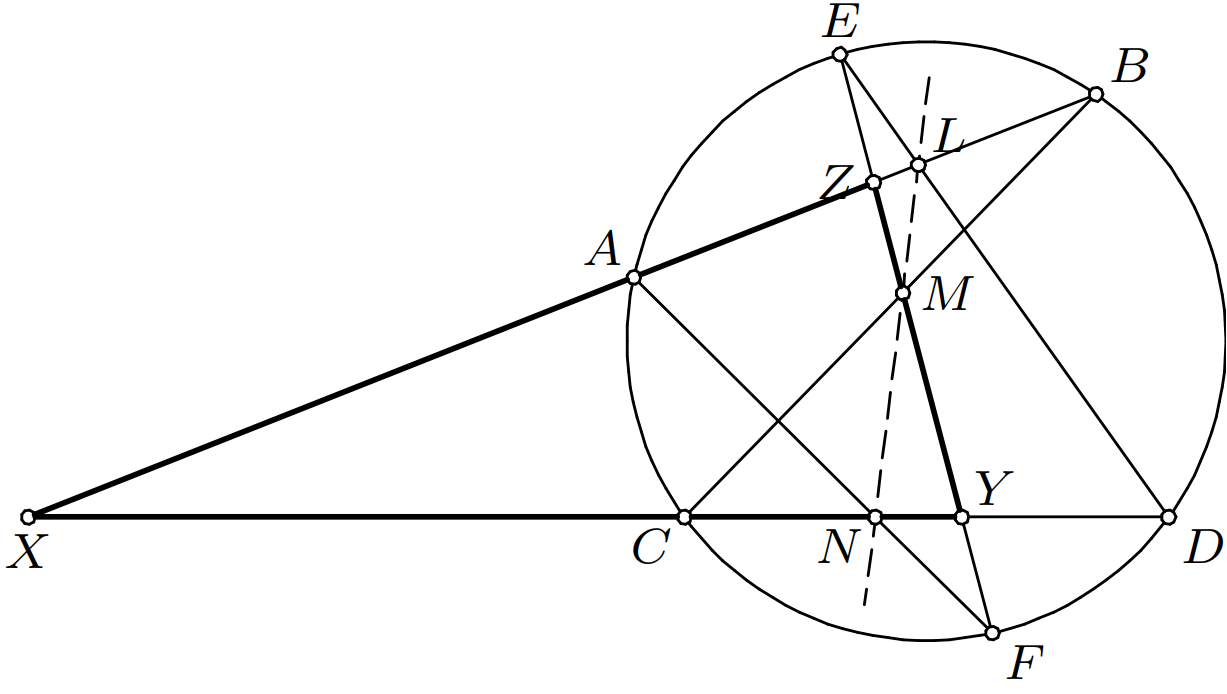
\includegraphics[scale=0.235]{Paskal}
\caption*{Slika 1.}
\end{wrapfigure}
\vspace{0.5cm}
\textbf{Dokaz:}
\vspace{0.5cm}
\\Neka se $AB$ i $CD$ seku u $X$, $CD$ i $EF$ u $Y$, a $EF$ i $AB$ u $Z$. Taqke $L, M, N$ lezhe na \text stranicama trougla $XYZ$, pa mozhemo da primenimo Menelajevu teoremu: treba pokazati da je $\D\frac{ZL}{LX}\cdot\frac{XN}{NY}\cdot\frac{YM}{MZ}=-1$. Radimo sa $\Delta XYZ$ kao baznim trouglom. Znamo da su taqke $L, D, E$ na pravoj, pa Menelajeva teorema daje $\D\frac{XD}{DY}\cdot\frac{YE}{EZ}\cdot\frac{ZL}{LX}=-1$. I taqke $C, M, B$ su \text kolinearne, pa imamo i $\D\frac{XC}{CY}\cdot\frac{YM}{MZ}\cdot\frac{ZB}{BX}=-1$. Najzad, taqke $N, F, A$ su kolinearne, pa je $\D\frac{XN}{NY}\cdot\frac{YF}{FZ}\cdot\frac{ZA}{AX}=-1$. Mnozhenjem ove tri jednakosti, koristec1i jednakosti potencije $XD\cdot XC = XB\cdot XA$, $YD\cdot YC = YF\cdot YE$ i $ZF\cdot ZE = ZB\cdot ZA$, dobijamo ono shto nam treba.\\
\begin{flushleft}
Paskalova teorema oqigledno ne zahteva da $ABCDEF$ bude konveksan shestougao, tako da su svi rasporedi tachaka dozvoljeni. Mozhemo da posmatramo i degenerisane sluchajeve, kada su neke dve prave paralelne ili se neke dve tachke poklapaju. Na primer, ako je $A = B$, za pravu $AB$ uzimamo tangentu na krug u $A$.\\[10mm]
\textbf{Zadaci:}\\[5mm]
\textbf{1.} Neka je $P$ taqka u unutrashnjosti trougla $ABC$. Oznaqimo sa $P_1$ i $P_2$ redom podnozhja
normala iz $P$ na $AC$ i $BC$, i sa $Q_1$ i $Q_2$ redom podnoжja normala iz $C$ na $AP$ i $BP$.
Dokazati da se prave $Q_1P_2$, $Q_2P_1$ i $AB$ seku u jednoj taqki.\\[5mm]
\textbf{2.} Trougao $ABC$ je upisan u krug G. Odabrana je taqka $M$ na simetrali ugla $A$, unutar
trougla. Prave $AM$, $BM$ i $CM$ ponovo seku Γ u $A_1$, $B_1$ i $C_1$ redom. Neka prava $A_1C_1$
seqe $AB$ u $P$, a $A_1B_1$ seqe $AC$ u $Q$. Dokazati da je $PQ\parallel BC$.\\[5mm]
\textbf{3.} U trouglu $ABC$, taqke $D$ i $E$ na pravoj $AB$ su takve da je $D-A-B-E$ i $AD = AC$,
$BE = BC$. Oznaqimo sa $M$ i $N$ redom sredixta lukova $AC$ i $BC$ opisanog kruga
$\Delta ABC$ koji ne sadrzhe trec1e teme. Prave $DM$ i $CA$ se seku u $P$, a prave $EN$ i $CB$
se seku u $Q$. Dokazati da centar upisanog kruga $I$ trougla $ABC$ lezhi na pravoj $PQ$.
\end{flushleft}
\newpage
\par
\begin{wrapfigure}[7]{r!}{0.35\textwidth}
\centering
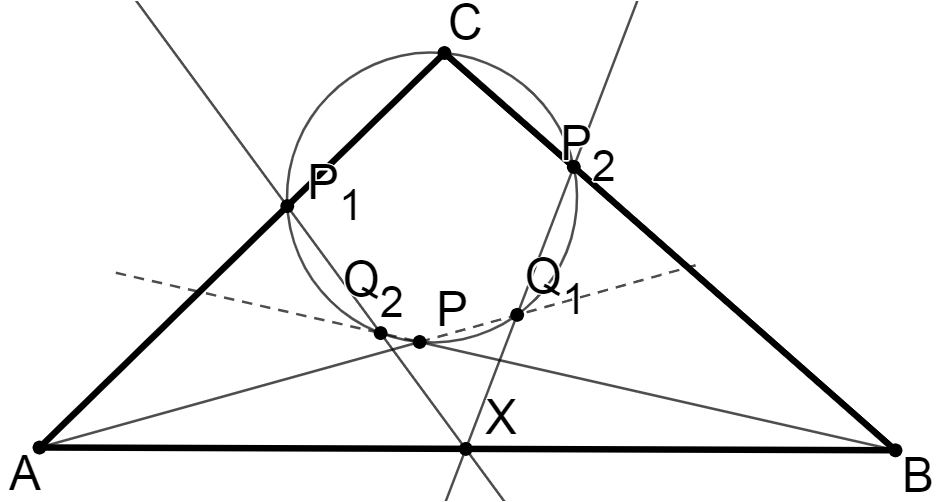
\includegraphics[scale=0.3]{Paskal1.PNG}
\caption*{Slika 2.}
\end{wrapfigure}
\textbf{Reshenja:}\\[5mm]
\textbf{1.} Taqke $P_1$, $P_2$, $Q_1$, $Q_2$ lezhe na krugu nad preqnikom $PC$. Po Paskalovoj teoremi u
xestouglu $P_1PP_2Q_1CQ_2$, taqke preseka parova pravih $P_1C$, $PQ_1$ (presek $A$), $P_1Q_2$, $P_2Q_1$
(presek $X$) i $PQ_2$, $P_2C$ (presek $B$) su \text kolinearne.\\[10mm]
\par
\begin{wrapfigure}[9]{r!}{0.35\textwidth}
\centering
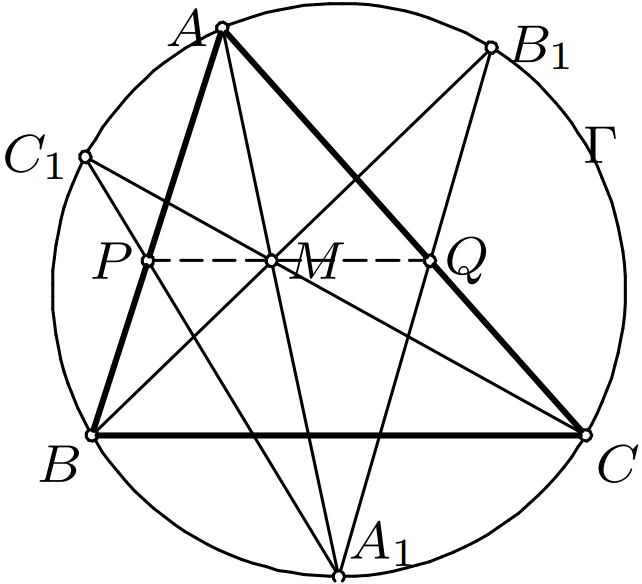
\includegraphics[scale=0.3]{Paskal2.PNG}
\caption*{Slika 3.}
\end{wrapfigure}
\textbf{2.} Na osnovu Paskalove teoreme na xestouglu $BACC_1A_1B_1$, taqke $P$, $Q$ i $M = BB1\cap CC1$ su \text kolinearne. Dalje, po uslovu zadatka, $A_1$ je sredixte luka $BC$, pa je tangenta $t$ u $A_1$ paralelna $BC$. Sada primenimo Paskalovu teoremu na $ABCC_1A_1A_1$: taqke $P = AB\cap A_1C_1$, $M = AA_1\cap CC_1$ i beskonaqna taqka $t\cap BC$ su na pravoj, tj. prave $t$, $BC$ i $PM$ \text pripadaju istom pramenu, xto znaqi da je $PM\parallel BC$, dakle \text{$PQ\parallel BC$}.\\[7mm]
\par
\begin{wrapfigure}[11]{r!}{0.43\textwidth}
\centering
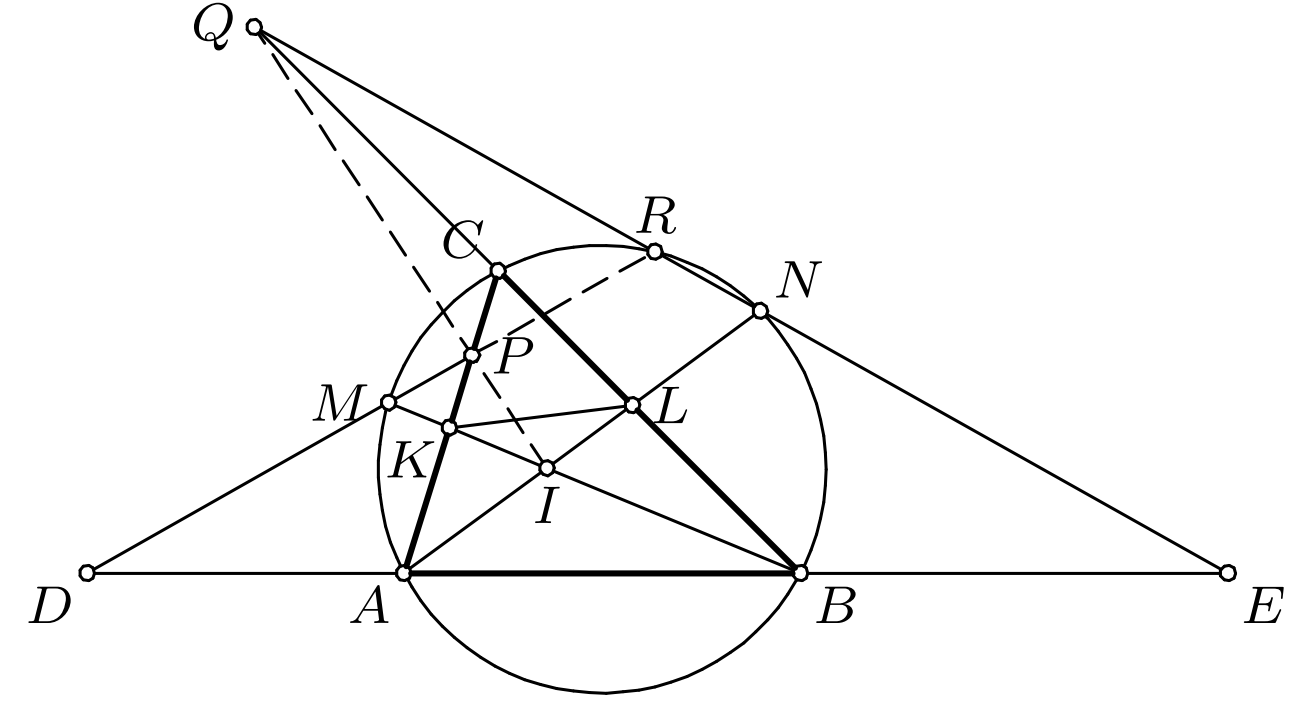
\includegraphics[scale=0.23]{Paskal3.PNG}
\caption*{Slika 4.}
\end{wrapfigure}
\textbf{3.} Neka $BM$ i $AN$ seku naspramne \text stranice trougla redom u $K$ i $L$. Iz sliqnosti \text trouglova $BCM$ i $BKA$ ($\ug BMC =\ug BAK$, \text{$\ug CBM =\ug KBA$}) imamo $BK \cdot BM = BA \cdot BC$; osim toga, zbog $CD\cap  AL$ vazhi $\D\frac{BA}{BD} =\frac{BL}{BC}$. Sledi $BK \cdot BM = BL \cdot BD$, xto zajedno sa $\ug DBM =\ug KBL$ daje $\Delta BDM \sim \Delta BKL$. Analogno, \text{$\Delta AEN\sim\Delta ALK$}. Neka se prave $DM$ i $EN$ seku u $R$. Dobijene sliqnosti daju $\ug RDE =\ug MDB =\ug LKB$ i $\ug DER =\ug AEN =\ug ALK$, tako da je $\ug NRM = 180^{\circ} - \ug RDE - \ug DER = 180◦ -\ug LKB - \ug ALK = \ug KIL = \ug BIA =  180^{\circ} - \ug IAB - \ug ABI = 180^{\circ} - \ug CAN - \ug MBC = \ug NCM$ (uglovi su orijentisani). Prema tome, $R$ je na opisanom krugu $\Delta ABC$. Sada kolinearnost taqaka $I$, $P$, $Q$ sledi iz Paskalove teoreme za taqke \text{$A$, $B$, $R$; $M$, $N$, $C$.}

\begin{thebibliography}{}
\bibitem{}D. Djukic1, \textit{Paskalova teorema, pol i polara}, \\\texteng{\url{https://imomath.com/srb/dodatne/paskalova%20teorema_ddj.pdf}}
\end{thebibliography}

\end{document}